\documentclass[12pt,a4paper]{article}

% --- Page Layout ---
\usepackage[top=1in, bottom=1in, left=0.85in, right=0.85in]{geometry}
\usepackage{setspace}
\doublespacing

% --- Paragraph Formatting ---
\usepackage{parskip}  % no paragraph indentation, adds vertical space
\setlength{\parskip}{0pt}  % resets indentation 
\setlength{\parindent}{15pt}  % resets indentation 
\usepackage{indentfirst}  % indent first paragraph of sections (optional)

% --- Font and Typography ---
\usepackage{newpxtext,newpxmath}
% \usepackage{times}
\usepackage[T1]{fontenc}
\usepackage[utf8]{inputenc}

% --- Section Title Formatting ---
\usepackage{titlesec}
\titleformat{\section}{\normalfont\Large\bfseries}{\thesection.}{1em}{}
\titleformat{\subsection}{\normalfont\large\bfseries}{\thesubsection.}{1em}{}

% --- Math ---
\usepackage{amsmath, amssymb, amsthm}

% --- Figures and Tables ---
\usepackage{graphicx}
\usepackage{caption}
\usepackage{subcaption}
\usepackage{float}
\usepackage{booktabs}
\usepackage{arydshln}

% --- References ---
% \usepackage{natbib}
% \usepackage[
%     backend=biber,
%     style=authoryear,
%     natbib=true
% ]{biblatex}
% \addbibresource{bibliography.bib}
\usepackage{natbib}
\bibliographystyle{apalike}

% --- Hyperlinks ---
\usepackage{hyperref}
\hypersetup{
    colorlinks=true,
    linkcolor=blue,
    citecolor=blue,
    urlcolor=blue
}

% --- Theorems ---
\newtheorem{theorem}{Theorem}
\newtheorem{proposition}{Proposition}
\newtheorem{lemma}{Lemma}

 % --- Header/Footer (optional for working papers) ---
% \usepackage{fancyhdr}
% \pagestyle{fancy}
% \fancyhead[L]{Working Paper}
% \fancyhead[R]{\thepage}

% --- Rotating tables ---
\usepackage{rotating} % Needed for sidewaystable

\title{Is Peru's FX Intervention Optimal? A Calibrated Framework}
\author{Gonzalo Bueno Bustíos}
\date{April 2025}

\begin{document}

\maketitle

\begin{abstract}
This essay evaluates the optimality of the Peruvian Central Bank's foreign exchange (FX) intervention policy using a calibrated version of the Itskhoki-Mukhin (2025) model. The model captures the trade-offs between stabilizing the exchange rate and minimizing distortions to output and risk-sharing. We calibrate the model to Peruvian data, including exchange rates, terms of trade, and capital flow shocks, and simulate counterfactual scenarios to assess the welfare implications of the actual FX policy. Our findings suggest that while the BCRP's interventions have reduced exchange rate volatility, they may have also introduced distortions that could be mitigated with a more targeted approach. The results highlight the importance of considering both macroeconomic stabilization and financial market frictions in designing optimal FX policies for emerging markets.
\end{abstract}

\newpage

\section{Introduction}

In recent years, due to significant movements of capital around the world, central banks have increasingly intervened in FX markets. This has raised questions regarding what the optimal FX policy to implement is. Does this policy maximize welfare? What are the optimal policy tools to implement it? Through what channels do these tools operate?

This essay analyzes the case of the Peruvian Central Bank (BCRP). The institution has been particularly active with FX interventions to reduce exchange rate volatility, through selling or buying USD or using financial products like bonds or swaps that keep international reserves untouched. This has been a success case. Compared to other countries in South America, Peru has had one of the lowest depreciations as well as lower volatility in recent years (see Figure \ref{fig:fx_plot}).

\begin{figure}[H]
    \centering
    \caption{FX Trends over time}
    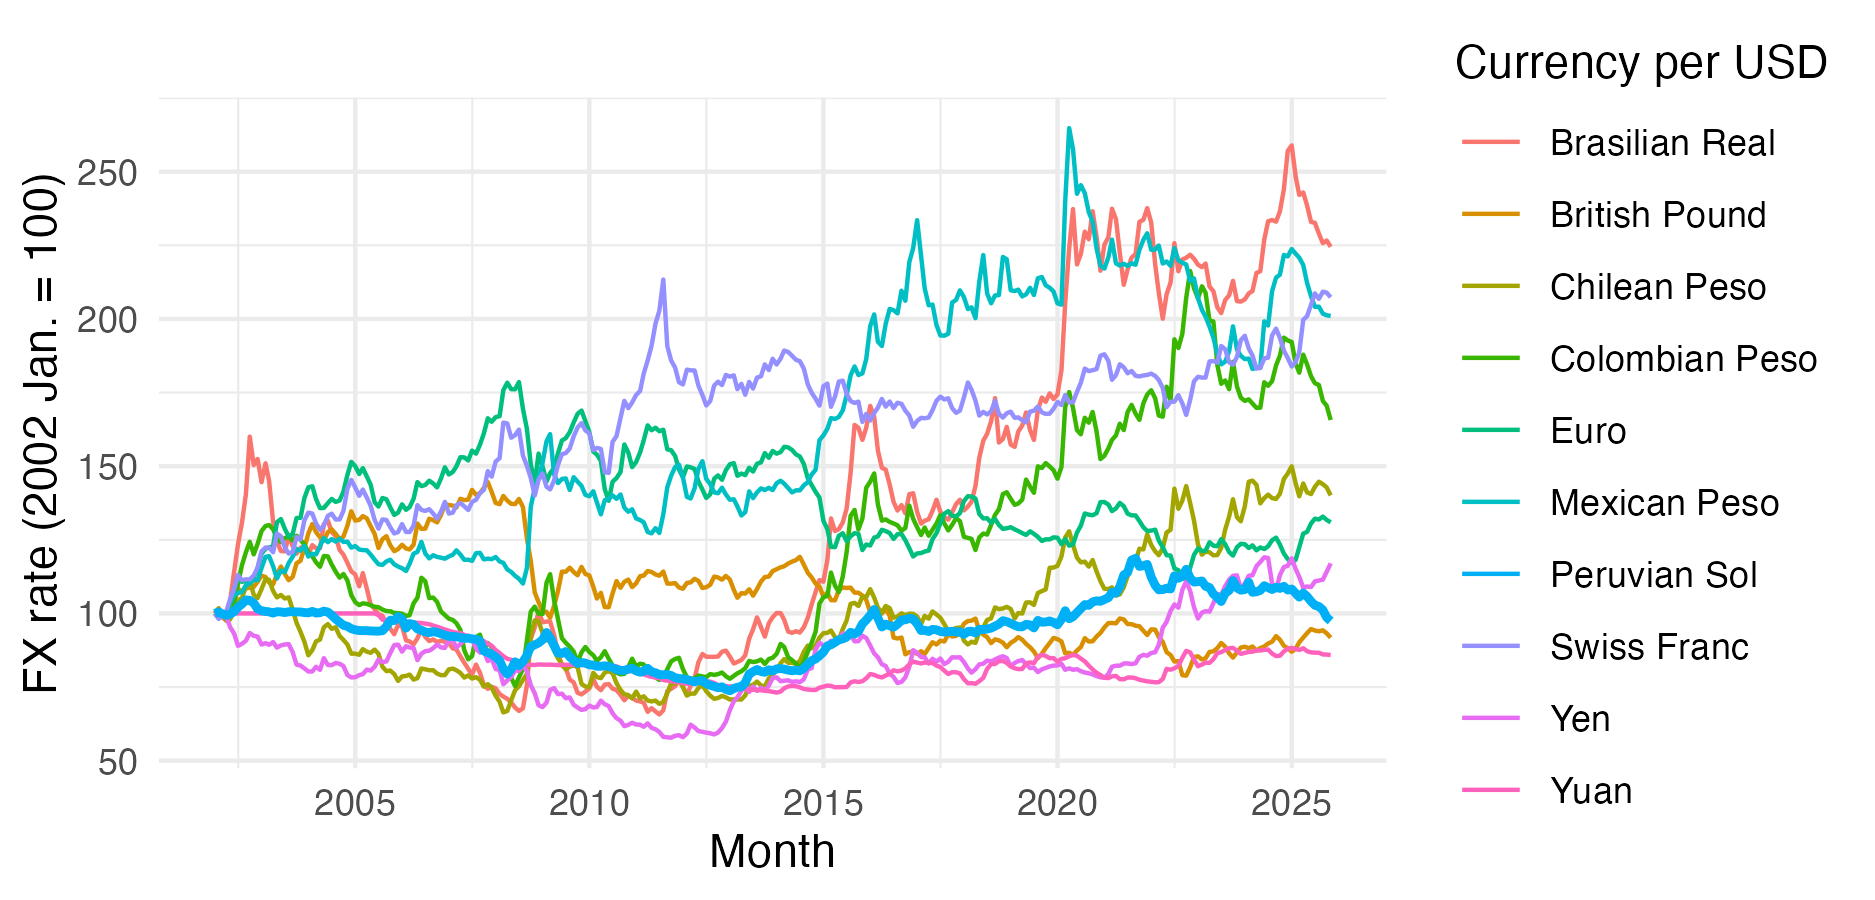
\includegraphics[width=\linewidth]{figures/fx_plot.png }     \label{fig:fx_plot}
    \smallskip
    \begin{minipage}{0.95\linewidth}
    \begin{singlespace}
    \footnotesize
    \textit{Notes:} This figure depicts the exchange rate per USD for ten economies from 2002 to 2025 normalized to January 2002 $= 100$. The thicker line corresponds to the Peruvian Sol (PEN), which has had the most stable value over the period. The sample includes the following countries: Peru, Brazil, Chile, Colombia, Mexico, Euro Area, Japan, UK, Switzerland, and China.
    \end{singlespace}
  \end{minipage}
 \end{figure}

From 2002 to 2025 (the period of Inflation Targeting in Peru), the volatility of the USD/Peruvian Sol (PEN) exchange rate has been 1.3\%\footnote{Measured as the standard deviation of log first-differences of the monthly exchange rate, multiplied by 100.}, while the average volatility of developed countries (excluding China, which has low volatility due to its exchange rate regime) and emerging economies is 1.7 and 2.4 times that of Peru, respectively. When taking into account inflation, the volatility of the real exchange rate is 1.32\%, with the corresponding ratios being 1.74 and 2.33 (see Table~\ref{tab:fx_volatility}).

%TC:ignore
\begin{table}[htbp]
  \centering
  \caption{Exchange Rate to USD Volatility}
  \label{tab:fx_volatility}
  \begin{tabular}{lcc}
    \toprule
    Currency & Nominal (\%) & Real (\%) \\
    \midrule
    Peruvian Sol  & 1.30 & 1.32 \\
    \midrule
    \multicolumn{3}{l}{\textit{Developed economies}} \\
    Euro          & 2.14 & -- \\
    Japanese Yen  & 2.29 & 2.35 \\
    British Pound & 2.15 & 2.26 \\
    Swiss Franc   & 2.20 & 2.28 \\
    Chinese Yuan  & 0.85 & 1.12 \\
    \midrule
    \multicolumn{3}{l}{\textit{Emerging economies}} \\
    Brazilian Real  & 3.78 & 3.75 \\
    Chilean Peso    & 2.74 & 2.61 \\
    Colombian Peso  & 3.23 & 3.20 \\
    Mexican Peso    & 2.76 & 2.73 \\
    \midrule
    \bottomrule
  \end{tabular}
  \smallskip
  \begin{minipage}{\linewidth}
    \small
    \textit{Notes:} Volatility is computed as the standard deviation of log
    first-differences of monthly bilateral exchange rates against the US dollar,
    multiplied by 100. Real exchange rates are constructed using consumer price
    indices. Sample period: 2002--2025.
  \end{minipage}
\end{table}
%TC:endignore

Maintaining this stability has been a particular challenge, as the Peruvian economy is a partially dollarized one (by September of 2025, 25.5 percent of credit issued to the private sector is in USD, see Figure \ref{fig:doll_plot}). Households and firms that hold these dollar debts are exposed to balance sheet effects: exchange rate swings translate into valuation shocks on dollar-denominated liabilities, tightening balance sheets and constraining spending. Moreover, the expectation of depreciation and rising domestic-currency debt service can trigger a sudden increase in the demand for dollars, pushing the exchange rate even further. This creates an incentive for the Central Bank to intervene in FX markets to dampen volatility.

The BCRP has been active in the FX market, intervening through spot transactions, bond operations (Certificado de Depósito Reajustable, CDRs), and exchange rate swap operations\footnote{This product created in 2014, allows agents to hedge their exchange rate exposure, while the BCR keeps international reserves untouched, as payments on differentials of exchange rates are made with domestic currency. For more details, see \cite{repec:rbp:moneda:moneda-170-02}.}. The total intervention as a percentage of GDP has varied over time, with peaks during periods of heightened volatility or external shocks (see Figure \ref{fig:fxi_plot}). The BCRP's intervention strategy has evolved, with a greater emphasis on sterilised operations to manage liquidity while influencing exchange rate dynamics. During the commodities supercycle, the BCRP accumulated reserves through purchases of USD. During the 2020 COVID-19 pandemic and the 2021 presidential elections, the BCRP significantly increased its intervention to mitigate volatility and support financial stability, reflecting its proactive approach in managing exchange rate risks in a partially dollarized economy.

\begin{figure}[H]
    \centering
    \caption{FX intervention rate}
    \includegraphics[width=0.85\linewidth]{figures/fxi_panel.png }     \label{fig:fxi_plot}
    \begin{minipage}{0.95\linewidth}
    \begin{singlespace}
    \footnotesize
    \textit{Notes:} This figure shows the FX intervention for the PEN/USD for the period 2002--2025. Top left: total intervention as a percentage of GDP. Remaining panels: the breakdown of the total intervention into net spot purchases of USD (top right), net bond operations (bottom left), and net swap operations (bottom right). Positive values indicate net USD purchases; negative values indicate net sales. Gray shading marks the 2020 COVID-19 shock and 2021 presidential elections.

    \end{singlespace}
  \end{minipage}
 \end{figure}

The case of Peru has already been subject to study. \cite{MONTORO2023102825} develop a New Keynesian small open economy model with segmented financial markets as in \cite{doi:10.1086/714447}. They derive closed-form solutions for optimal FX intervention and show that the optimal policy prescribes leaning against the wind in response to portfolio flow shocks but leaning with the wind in response to fundamental shocks. This implies that simple exchange rate stabilisation rules are not generally optimal. Under a general parametrisation, even fundamental shocks activate the portfolio balance channel, causing the exchange rate to deviate from its efficient path. Using a Bayesian VAR estimated on Peruvian data, they find empirical support for BCRP intervention responding to both types of shocks. 

The research question of this essay is: has the FX policy of the Peruvian Central Bank been optimal? This essay builds on the framework of \cite{itskhokimukhin2025}, where an optimal FX intervention policy is derived and the welfare losses originating from deviations from the first-best allocation are quantified. Differently from \cite{MONTORO2023102825}, who evaluate simple implementable rules, I contrast the BCRP's actual intervention behaviour against the fully optimal policy benchmark from \cite{itskhokimukhin2025}, and different rule variations to quantify the resulting welfare gap.

This essay is structured as follows. Section~\ref{sec:literature_review} reviews the existing literature. Section~\ref{sec:theoretical_framework} introduces the theoretical framework used to evaluate the optimality of FX policy. Section~\ref{sec:data_and_calibration} describes the data and calibration strategy. Section~\ref{sec:tests} presents the empirical tests. Section~\ref{sec:results} reports the results of the model simulations and empirical estimations. Finally, Section~\ref{sec:conclusions} concludes.

\section{Literature review}
\label{sec:literature_review}



\section{Theoretical framework}
\label{sec:theoretical_framework}

This section introduces the model that will be used in the essay. It follows the \cite{itskhokimukhin2025} model that captures the policy decision of a Central Bank over the use of monetary policy and FX interventions. The model is described in a general form, with the specific equations that are relevant to the model built for calibration and simulation.

\subsection{The economy}

The model describes a small open economy with four types of agents: households, arbitrageurs (financial intermediaries), noise traders, and a government that includes the central bank. The key feature is segmentation in global asset markets: domestic households have access only to local-currency bonds, so all international capital flows must be intermediated by the arbitrageurs. This segmentation is what generates endogenous deviations from uncovered interest rate parity (UIP) and creates a role for FX intervention. 

\paragraph{Households.} A representative household derives utility from consumption of non-tradable goods $C_{Nt}$ and tradable goods $C_{Tt}$
\begin{equation}
    U_t = \gamma \log C_{Tt} + (1-\gamma) \log C_{Nt},
    \label{eq:utility}
\end{equation}
where $\gamma \in (0,1)$ measures the openness of the economy, i.e.\ the weight placed on tradable consumption. The household supplies labor inelastically to non-tradable production and receives profits from firms. Crucially, the household can only save and borrow using the home-currency bond $B_t$ at the domestic nominal interest rate $R_t$; it has no direct access to foreign-currency assets.

\paragraph{Goods market.} Non-tradable output $Y_{Nt} = C_{Nt}$ clears domestically. Under fully sticky non-tradable prices ($P_{Nt} = 1$) and the law of one price for tradables ($P_{Tt} = E_t P^*_{Tt}$), the optimal expenditure allocation between tradables and non-tradables implies:
\begin{equation}
    E_t = \frac{\gamma}{1-\gamma} \cdot \frac{C_{Nt}}{C_{Tt}},
    \label{eq:expenditure}
\end{equation}
so that the nominal exchange rate $E_t$ is the relative price that clears the goods market.

\paragraph{Financial intermediaries (arbitrageurs).} Arbitrageurs can hold both home and foreign currency bonds, but face a mean-variance portfolio problem with risk-aversion parameter $\omega > 0$. Their optimal carry-trade position $D^*_t/R^*_t$ satisfies
\begin{equation}
    \frac{D^*_t}{R^*_t} = \frac{\mathbb{E}_t[\Theta_{t+1}\tilde{R}^*_{t+1}]}{\omega \sigma^2_t},
    \label{eq:arbitrageur}
\end{equation}
where $\Theta_{t+1} = \beta C_{Tt}/C_{Tt+1}$ is the stochastic discount factor of households, $\tilde{R}^*_{t+1} = R^*_t - R_t E_t/E_{t+1}$ is the return on one dollar of carry trade, and $\sigma^2_t \equiv \text{var}_t(\Delta e_{t+1})$ is the conditional exchange rate variance. As $\omega \to 0$ the market becomes frictionless and UIP holds exactly. For $\omega > 0$, arbitrageurs demand a risk premium in proportion to both their net exposure and the level of exchange rate volatility, which is the core friction of the model.

\paragraph{Noise traders and the government.} Noise traders generate exogenous currency demand shocks $N^*_t$ that represent non-fundamental capital flows. The government (central bank) holds net foreign currency assets $F^*_t$ via sterilised FX interventions. Financial market clearing requires:
\begin{equation}
    D^*_t + F^*_t + N^*_t = B^*_t,
    \label{eq:fmclearing}
\end{equation}
where $B^*_t$ is the net foreign asset (NFA) position of domestic households intermediated through the financial sector. Sterilisation means that FX purchases or sales by the central bank do not affect the domestic monetary base.%, so they work purely through the portfolio-balance channel: by absorbing or injecting foreign currency supply, the government shifts the net exposure borne by arbitrageurs and thus changes the risk premium they demand.

\paragraph{First-best allocation and risk-sharing wedge.} The first-best allocation $\{\tilde{C}_{Nt}, \tilde{C}_{Tt}, \tilde{B}^*_t\}$ is defined as the equilibrium that obtains when $\omega = 0$, so that UIP holds and households can smooth tradable consumption at the world interest rate~$R^*_t$. 

Deviations from this benchmark are captured by two wedges: the \textit{output gap} $x_t \equiv \log(C_{Nt}/\tilde{C}_{Nt})$, which measures the cost of nominal rigidities in the goods market, and the \textit{risk-sharing wedge} $z_t \equiv \log(C_{Tt}/\tilde{C}_{Tt})$, which measures the distortion to tradable consumption caused by financial frictions. When $z_t < 0$, households consume fewer tradables than is socially optimal because arbitrageurs charge a premium for intermediating capital flows; when $z_t > 0$ the opposite holds.

The frictional UIP condition (obtained by combining household and arbitrageur optimality with financial market clearing) shows that the expected change in the risk-sharing wedge equals the UIP deviation:
\begin{equation}
    i_t - i^*_t - \mathbb{E}_t \Delta e_{t+1} = \mathbb{E}_t \Delta z_{t+1},
    \label{eq:uip_wedge}
\end{equation}
so the risk-sharing wedge and the UIP premium are two sides of the same friction: the risk premium charged by arbitrageurs is precisely what prevents households from achieving efficient risk sharing.

\subsection{The policy problem}

The Central Bank has two tools to intervene in the economy: (1) a standard interest rate policy, and (2) an FX intervention that can absorb shocks that create deviations from UIP due to capital flows in the financial market. The Central Bank minimizes a loss function between the output gap (or a measure that relies on sticky prices, such as actual inflation relative to the target) and a wedge that measures deviations from UIP subject to the constraints of the economy. \cite{itskhokimukhin2025} presents the policy problem as deviations from a first-best allocation.

The loss function is given by a second-order approximation of the household welfare around the first-best allocation:

\begin{equation}
    L = \frac{1}{2}\mathbb{E}\sum_{t=0}^{\infty} \beta^t \left[ \gamma z_t^2 + (1-\gamma) x_t^2 \right]
\end{equation}

where $z_t$ is the risk sharing wedge and $x_t$ is the output gap, $\beta$ is the discount factor, and $\gamma$ is a parameter that captures openness of the economy.

The constraints from the economy solution are:

\begin{itemize}

    \item \textit{Country budget constraint} (exports-imports as counterpart of the net foreign asset position): 
    $\beta b_t^* = b_{t-1}^* - z_t$.
    
    \item \textit{Expenditure allocation condition} in the goods market: 
    $e_t = \tilde{q}_t + x_t - z_t$.
    
    \item \textit{Equilibrium in the financial market}:
    $\mathbb{E}_t \Delta (z_{t+1}) = \bar{\omega} \bar{\sigma}^2_t (n_t^* + f_t^* - b_t^*)$.

\end{itemize}

The first-best allocation is achieved when $z_t = 0$ and $x_t = 0$ for all $t$. Any additional constraints on the FX intervention will create deviation from the best-case scenario. A simplification of the framework model is that the volatility of the exchange rate $\bar{\sigma}^2_t$ is treated as a constant across time and states, determined by a fixed-point condition $\bar{\sigma}^2 = \text{Var}(\Delta e_{t+1})$. This allows for a simple numerical solution while matching the data properties.

The Ramsey optimal monetary policy for any given FX intervention rule satisfies the following conditions:

\begin{itemize}
    \item \textit{Output gap:} $x_{t+1} = -\delta_t (e_{t+1} - \mathbb{E}_t e_{t+1})$.
    \item \textit{Intensity of monetary policy lean:}
    \[ \delta_t = \frac{2\gamma\bar{\omega}}{1-\gamma} \cdot \frac{\bar{\omega}\bar{\sigma}^2_t}{1 + \beta + \bar{\omega}\bar{\sigma}^2_t} \cdot (n_t^* + f_t^* - b_t^*). \]
\end{itemize}
    
This corresponds to the optimal policy response when FX interventions are constrained. In the case of the Peruvian Central Bank, there is a limit in both the amount of reserves available as well as the amount of information available to compensate for noise shocks that lead to increased volatility. This can be interpreted as an FX intervention rule $f_t^* = -\phi\, n_t^*$, where $\phi$ governs the degree to which the central bank offsets exogenous currency demand shocks through sterilised FX interventions. %The monetary interest rate movements can be recovered from the path of UIP deviations: $i_t - i_t^* - \mathbb{E}_t \Delta e_{t+1} = \mathbb{E}_t \Delta (z_{t+1})$.

\subsection{Model Equations}

The linearised model consists of the following system of equations:

\begin{singlespace}

\textbf{Exchange rate determination (goods market clearing):}
\begin{equation}
    e_t = \tilde{q}_t + x_t - z_t
    \label{eq:er}
\end{equation}

\medskip
\textbf{NFA dynamics (budget constraint):}
\begin{equation}
    \beta b^*_t = b^*_{t-1} - z_t
    \label{eq:nfa}
\end{equation}

\medskip
\textbf{Risk-sharing condition (financial market clearing):}
\begin{equation}
    \mathbb{E}_t \Delta z_{t+1} = \bar{\omega}\,\bar{\sigma}^2
    \left(n^*_t + f^*_t - b^*_t\right)
    \label{eq:risksharing}
\end{equation}

\medskip
\textbf{Exchange rate volatility:}
\begin{equation}
    \bar{\sigma}^2 = \text{Var}\left(\Delta e_{t+1}\right)
    \label{eq:sigma}
\end{equation}

\medskip
\textbf{Output gap:}
\begin{equation}
    x_{t+1} = -\delta_t \left(e_{t+1} - \mathbb{E}_t e_{t+1}\right)
    \label{eq:outputgap}
\end{equation}

\medskip
\textbf{Intensity of monetary policy lean:}
\begin{equation}
    \delta_t = \frac{2\gamma\bar{\omega}}{1-\gamma}
    \cdot \frac{\bar{\omega}\bar{\sigma}^2_t}{1 + \beta + \bar{\omega}\bar{\sigma}^2_t}
    \cdot \left(n^*_t + f^*_t - b^*_t\right)
    \label{eq:delta}
\end{equation}

\medskip
\textbf{Terms-of-trade shock:}
\begin{equation}
    \tilde{q}_t = \rho_q\, \tilde{q}_{t-1} + \varepsilon^q_t
    \label{eq:qtilde}
\end{equation}

\medskip
\textbf{Capital flow shock:}
\begin{equation}
    n^*_t = \rho_n\, n^*_{t-1} + \varepsilon^n_t
    \label{eq:nstar}
\end{equation}

\medskip
\textbf{FX intervention rule (partial offset):}
\begin{equation}
    f^*_t = -\phi\, n^*_t
    \label{eq:fxi}
\end{equation}

\end{singlespace}

\section{Data and calibration}
\label{sec:data_and_calibration}

\subsection{Data sources}

The empirical analysis draws on quarterly data for Peru covering the period 2002Q1--2025Q2, which spans the full inflation-targeting regime of the Banco Central de Reserva del Per\'u (BCRP). All series are obtained from the BCRP's public statistical database unless otherwise noted.

The following variables are used. The \textit{nominal exchange rate} is the quarterly average PEN/USD spot rate. \textit{FX intervention volumes} are measured as BCRP net spot purchases of US dollars, bond and swap opreations (as percentage of GDP), with negative values indicating net USD sales. The \textit{terms of trade} index is constructed from export and import price indices and serves as the primary proxy for the fundamental shock $\tilde{q}_t$. \textit{Gross domestic product} is real quarterly GDP (base year 2007). The \textit{trade balance} is measured as a share of GDP. The \textit{interest rate} from both the BCRP and FED is used as the domestic and foreign rates for the UIP. The \textit{expectations of the exchange rate} are recovered from expectations surveys for 12 months ahead done by the BCRP. This is the only variable available from december 2016.

\subsection{Calibration}

Several parameters of the model are set using a combination of standard values from the literature on small open economies, Peru-specific estimates, and data moments. Table~\ref{tab:calibration} summarises the baseline calibration.

\paragraph{Preference parameters.} The discount factor is set to $\beta = 0.995$, consistent with literature for quarterly models. The openness parameter $\gamma$ is calibrated to match the share of tradable consumption in total spending; using BCRP national accounts data this yields $\gamma \approx 0.27$.

\paragraph{Financial friction.} The key parameter $\bar{\omega} = \omega_0 \bar{Y}_T / \beta$ governs the price of FX risk. The transmition of shocks from noise traders, capital flows or FX interventions is scaled by $\bar{\omega} \bar{\sigma}^2$. In other words, it determines the strength of the portfolio-balance channel and therefore the welfare gains from FX intervention. Obtaining a Peru-specific estimate is central, as it will allow to recover the noise trader shocks from observed data. The parameter $\omega_0$ is calibrated to $100$, which, together with $\bar{\sigma}^2 = 0.000525$ from the variance of log-differences over quarterly data, yield a coefficient $\bar{\omega} \bar{\sigma}^2 = 0.0525$. A high value of $\bar{\omega}$ would give too much weight to the FX interventions over the explanation of exchange rate movements, which would require a spurious noise trader shock identification to compensate.

\paragraph{Shock processes.} The persistence and standard deviation of the terms-of-trade shock $(\rho_q, \sigma_q)$ are estimated by fitting an AR(1) to the HP-filtered log terms-of-trade series. This yields $\hat{\rho}_q \approx 0.84$ and $\hat{\sigma}_q \approx 0.0384$. In the model, shocks to $\tilde{q}_t$ have a direct impact on the exchange rate, so it would be inaccurate to assume that the recovered moments from the HP filter are representative of the effect of terms-of-trade shocks on the exchange rate. Indeed, when noise trader shocks are turned off, the resulting fixed-point exchange rate volatility exceeds the observed volatility in the data. 

To address this, I estimate a log-difference regression of the exchange rate on the terms of trade and use the resulting pass-through coefficient ($0.1237$) to scale the volatility of $\tilde{q}_t$ shocks down to $\sigma_q \approx 0.0047$ (see Table~\ref{tab:tot_passthrough} and Figure~\ref{fig:tot_passthrough_plot}). This pass-through regression is a reduced-form approximation that does not address the joint endogeneity of the exchange rate and terms of trade; a structural identification is beyond the scope of this essay, but the resulting calibration produces model-implied exchange rate volatility consistent with the data.

The persistence and standard deviation of the capital flow shock $(\rho_n, \sigma_n)$ are calibrated to match $\bar{\sigma}^2 = 0.000525$. In other words, it is calibrated based on the residual standard deviation from the exchange rate. This yields $\hat{\rho}_n = 0.9285$ and $\hat{\sigma}_n = 0.1544$.

\paragraph{FX intervention intensity.} The FXI intensity coefficient $\phi$ is calibrated by matching the observed standard deviation of FX intervention $\sigma_{f^*} \approx 0.067$. Taking variances on both sides of equation~\eqref{eq:fxi} and using the unconditional variance of the AR(1) process for $n^*_t$, the coefficient is recovered as $\phi = \sigma_{f^*}\sqrt{1 - \rho_n^2}/\sigma_n$. In this way, $\phi$ is the ratio of FXI volatility to noise trader volatility. It captures the proportion of capital flow shocks that the central bank absorbs through intervention. The calibration of the noise trader shocks therefore governs the implicit FX intervention intensity. A value of $\hat{\phi} = 0.16$ implies that the BCRP offsets around 16\% of the capital flow shocks hitting the economy, compared to the optimal $\phi^* = 1$ predicted by the first-best intervention rule. The resulting estimate is reported in Table~\ref{tab:calibration}.

\begin{table}[H]
    \centering
    \begin{singlespace}
    \caption{Baseline calibration}
    \label{tab:calibration}
    \begin{tabular}{llrl}
        \toprule
        Parameter & Symbol & Value & Source \\
        \midrule
        Discount factor & $\beta$ & 0.995 & Standard \\
        Openness & $\gamma$ & 0.27 & National accounts \\
        FX risk price & $\bar{\omega}$ & 100 & Calibrated \\
        Exchange rate variance & $\bar{\sigma}^2$ & 0.000525 & Sample variance of $\Delta e_t$ \\
        ToT persistence & $\rho_q$ & 0.84 & AR(1) on HP-filtered ToT \\
        ToT shock s.d. & $\sigma_q$ & 0.0047 & AR(1) on HP-filtered ToT \\
        Capital flow persistence & $\rho_n$ & 0.93 & Moment matching \\
        Capital flow shock s.d. & $\sigma_n$ & 0.15 & Moment matching \\
        Intervention intensity & $\phi$ & 0.16 & Moment matching \\
        \bottomrule
    \end{tabular}
    \end{singlespace}
\end{table}

\subsection{Model estimation}

The linearised equilibrium system -- equations~\eqref{eq:er}--\eqref{eq:fxi} -- is treated as a DSGE model with one non-linear fixed-point equation for $\bar{\sigma}^2$ that requires iterative solution. The fixed-point iteration proceeds as follows: given a conjectured value for $\bar{\sigma}^2$ (which is the sample estimate), the model is solved in Dynare, and the implied variance of $\Delta e_{t+1}$ is calculated from the theoretical variance and first autocorrelation of $e_t$.\footnote{Since Dynare reports theoretical moments of levels, the variance of exchange rate changes is recovered as $\bar{\sigma}^2 = 2\,\text{Var}(e)(1 - \rho_e)$, where $\rho_e$ is the first-order autocorrelation of $e_t$. This follows from stationarity: $\text{Var}(\Delta e) = \text{Var}(e_{t+1}) + \text{Var}(e_t) - 2\,\text{Cov}(e_{t+1}, e_t) = 2\,\text{Var}(e)(1 - \rho_e)$.} The implied variance is compared to the conjectured value; if the difference is below a tolerance of $10^{-7}$, the process terminates. Otherwise, the conjecture is updated with damping, that is, the new conjecture is a weighted average of the implied estimate and the previous value, $\bar{\sigma}^2_{\text{next}} = \alpha\, \bar{\sigma}^2_{\text{new}} + (1-\alpha)\, \bar{\sigma}^2_{\text{old}}$ with $\alpha = 0.4$, to prevent overshooting, and the iteration continues.

The calibration is performed on the crawling peg regime ($f^*_t = -\phi\, n^*_t$), as this is the relevant regime that can be matched to data. The resulting fixed-point $\bar{\sigma}^2$ is then used as an input for the first-best and free float regimes, where the algorithm obtains regime-specific exchange rate volatility. This is necessary because changes in the intervention rule alter exchange rate dynamics, so the data moment matching would not be appropriate for the counterfactual regimes.

Five policy regimes are simulated and compared:

\begin{enumerate}
    \item \textbf{Crawling peg/Partial intervention} ($\phi = \hat{\phi}$): the central bank offsets only a fraction $\hat{\phi}$ of capital flow shocks, matching estimated BCRP behaviour. This is the empirically relevant regime and generates a welfare loss intermediate between the first-best and the free float.
        
    \item \textbf{First-best intervention} ($\phi = 1$): the central bank fully offsets capital flow shocks, $f^*_t = -n^*_t$, and uses monetary policy to close the output gap. This achieves $z_t = x_t = 0$ and represents the welfare benchmark.

    \item \textbf{Free float} ($\phi = 0$, $f^*_t = 0$): no FX intervention. Shocks are absorbed by the exchange rate and the risk-sharing wedge.
    
    \item \textbf{Fixed exchange rate via monetary policy} ($\phi = 0$, $e_t = 0$): the central bank pegs the exchange rate through the interest rate, so that $x_t = z_t - \tilde{q}_t$. $\bar{\sigma}^2$ is set to a small nonzero value ($2 \times 10^{-4}$, approximately 38\% of the crawling peg estimate) to preserve the financial friction channel while keeping the exchange rate effectively fixed. The welfare cost comes primarily from the output gap absorbing terms-of-trade shocks, with a residual contribution from capital flow shocks through the still-active risk premium. No fixed-point iteration is performed.
    
    \item \textbf{Fixed exchange rate via FX intervention} ($e_t = 0$, $\bar{\sigma}^2 > 0$): the central bank fixes the exchange rate through intervention, setting $f^*_t$ such that $e_t = 0$ in equilibrium. $\bar{\sigma}^2$ is calibrated to the crawling peg sample estimate ($5.25 \times 10^{-4}$), preserving the full financial friction channel: arbitrageurs still price currency risk, so $n^*_t$ shocks affect the risk-sharing wedge even though the exchange rate does not move. This can be interpreted as a peg with imperfect credibility or limited reserves. If the policy were to break down, the exchange rate would adjust, and market participants price this residual risk. The resulting model-implied exchange rate volatility is zero, but the welfare losses reflect the cost of maintaining the peg through active intervention.

\end{enumerate}

\section{Empirical Tests}
\label{sec:tests}

This section presents an empirical test of the model's predictions using Peruvian data, followed by a welfare comparison across policy regimes.

\subsection{Test 1: UIP deviations and the financial friction mechanism}

The \cite{itskhokimukhin2025} model predicts that UIP deviations are driven by the frictional risk premium $\bar{\omega}\bar{\sigma}^2 D^*_t$, where $D^*_t \equiv n^*_t + f^*_t - b^*_t$ is the net currency exposure absorbed by arbitrageurs. FX intervention changes $D^*_t$ and therefore the risk premium. A model without financial market segmentation ($\bar{\omega} = 0$) predicts no relationship between intervention and UIP deviations.

\paragraph{Step 1: Documenting the UIP puzzle for Peru.} I estimate the standard UIP regression:
\begin{equation}
    \Delta e_{t+1} = \alpha + \beta_1 (i_t - i^*_t) + \varepsilon_{t+1},
    \label{eq:uip_classic}
\end{equation}
where $\Delta e_{t+1}$ is the expected log change in the PEN/USD rate, $i_t$ is the BCRP reference rate, and $i^*_t$ is the US federal funds rate. UIP predicts $\beta_1 = 1$ and $\alpha = 0$.

\paragraph{Step 2: Testing the portfolio balance channel.} I test whether BCRP intervention is related to UIP deviations, as predicted by the portfolio balance channel. Define the UIP deviation $\hat{\psi}_{t} \equiv \mathbb{E}_t \Delta e_{t+1} - (i_t - i^*_t)$, which equals $-\bar{\omega}\bar{\sigma}^2(n^*_t + f^*_t - b^*_t)$ in the model. I estimate:
\begin{equation}
    \hat{\psi}_{t} = \alpha + \beta_2\, f^*_{t} + \beta_3\, f^*_{t-1} + \varepsilon_{t},
    \label{eq:uip_fxi}
\end{equation}

where $f^*_{t}$ is BCRP net spot purchases as a percentage of GDP. The model has two predictions: (i) FX interventions reduce UIP deviations by altering the risk premium and (ii) as shocks hit the exchange rate, interventions respond countercyclically to the shock but procyclically with respect to UIP deviations, as both are driven by $n^*_t$. Substituting the policy rule $f^*_t = -\phi n^*_t$ into the UIP deviation yields $\hat{\psi}_t = -\bar{\omega}\bar{\sigma}^2\left(\frac{1-\phi}{\phi}f^*_t + b^*_t\right)$. The component $-\bar{\omega}\bar{\sigma}^2 f^*_t$ captures the direct effect of intervention on the risk premium, while $\bar{\omega}\bar{\sigma}^2\frac{1}{\phi}f^*_t$ captures the policy response to $n^*_t$.

The contemporaneous $\beta_2$ picks up the procyclical relationship: when a capital flow shock hits, both the deviation and the intervention move in the same direction, as the BCRP reacts to the same shock driving the deviation. So $\beta_2 > 0$. The lagged $\beta_3$ picks up the direct effect of intervention on UIP deviations. Since $f^*_{t-1}$ was set before $n^*_t$ is realised, and the contemporaneous regressor absorbs the $n^*_t$ signal, the lag captures how intervention affects the risk premium: by reducing arbitrageur exposure $D^*_{t-1}$, past intervention compresses the risk premium going into the current period. So $\beta_3 < 0$.

It is worth noting that this identification strategy has limitations. The regression cannot cleanly separate the structural effect of intervention from the reaction function, as both $f^*_t$ and $\hat{\psi}_t$ are jointly determined by the same unobserved shocks. The inclusion of the lag helps, but $b^*_t$ remains omitted and is likely correlated with intervention. Additionally, the relationship between FXI and UIP deviations is not stable across the sample. These results should therefore be interpreted as suggestive evidence consistent with the portfolio balance channel, not as a structural identification of $\bar{\omega}\bar{\sigma}^2$.

\subsection{Test 2: Welfare comparison across policy regimes}

This test compares the welfare loss with respect to the first best for the five policy regimes described in Section~\ref{sec:data_and_calibration}. Additionally, I include the actual BCRP policy path. I focus on the 2020--2021 period, which includes the COVID-19 shock and the 2021 presidential elections, as this is a period of high volatility and heavy intervention where the welfare losses from suboptimal policy are likely to be more visible. 

\paragraph{Shock recovery.} To input historical shocks through the model under different policy regimes, I first need to recover the unobserved shock sequences. I modify the crawling peg model to include an error in the FX intervention rule: $f^*_t = -\phi\, n^*_t + \varepsilon^f_t$, where $\varepsilon^f_t$ captures deviations from the estimated partial intervention rule. The model has three shocks ($\varepsilon^q_t$, $\varepsilon^n_t$, $\varepsilon^f_t$) and three observables: the HP-filtered log terms of trade $\tilde{q}_t$, the log-difference of the exchange rate $\Delta e_t$, and FX intervention $f^*_t$. The HP-filtered exchange rate is used rather than the raw series because the model defines variables as log-deviations from the first-best allocation. The persistent trend in the observed exchange rate is not consistent with the model's stationary structure. Using the calibrated parameters from Table~\ref{tab:calibration}, I apply the Kalman smoother to recover the smoothed state variables, including $z_t$, $n^*_t$, and $b^*_t$, as well as the structural shock sequences. 

\paragraph{Counterfactual simulation.} With the recovered $\varepsilon^q_t$ and $\varepsilon^n_t$ sequences, I simulate the 2020--2021 episode under each policy regime. The decision rules from the linearised model are used to compute the paths of $z_t$, $x_t$, $e_t$, and $f^*_t$. The conditional welfare loss is computed as:
\begin{equation}
    \mathcal{L} = \frac{1}{2} \sum_{t=0}^{T} \beta^t \left[\gamma z_t^2 + (1-\gamma) x_t^2\right],
    \label{eq:welfare_cond}
\end{equation}
where $T$ covers the 2020Q1--2023Q4 window (16 quarters). This finite-horizon conditional welfare measure captures the cost of each regime during the crisis episode.

For the BCRP actual policy, I use the recovered smoothed paths of $z_t$ and $x_t$, which reflect the actual intervention volumes and exchange rate dynamics observed during the period. This allows a direct comparison between what the BCRP did and what each counterfactual regime would have delivered given the same underlying shocks.

It is worth noting that the shock recovery is not a structural identification of the noise trader shocks. They are inferred from the model's equilibrium conditions and the estimated parameters, not directly observed. The resulting shock series should be interpreted as the model's best approximation of the unobserved shocks consistent with observed data. A more complete exercise would model the FX policy rule to account for reserve accumulation during high export price periods and responses to changes in $b^*_t$, but that is beyond the scope of this essay.

\section{Results}
\label{sec:results}

\subsection{Estimation results}

 \begin{figure}[H]
    \centering
    \caption{Impulse response to a one-standard-deviation terms-of-trade shock}
    \includegraphics[width=\linewidth]{figures/IRF_ToT_shock.pdf}     
    \label{fig:IRF_ToT_plot}
 \end{figure}


\begin{figure}[H]
    \centering
    \caption{Impulse response to a one-standard-deviation capital flows shock}
    \includegraphics[width=\linewidth]{figures/IRF_CapFlow_shock.pdf}  
    \label{fig:IRF_CapFlow_plot}
 \end{figure}
 
 \subsection{Test 1: UIP deviations and the financial friction mechanism}


 \subsection{Test 2: Welfare comparison across policy regimes}

 \begin{figure}[H]
    \centering
    \caption{Decomposition of the actual BCRP policy}
    
\includegraphics[width=1\linewidth]{figures/fstar_decomposition.pdf}  
    \label{fig:fstar_decomposition_plot}
 \end{figure}


\section{Conclusions}
\label{sec:conclusions}

[To be completed.]

\newpage

%TC:ignore

\appendix
\section{Appendix}

\setcounter{figure}{0}
\renewcommand{\thefigure}{A\arabic{figure}}

\setcounter{table}{0}
\renewcommand{\thetable}{A\arabic{table}}


\begin{figure}[H]
    \centering
    \caption{Dollarization rate}
    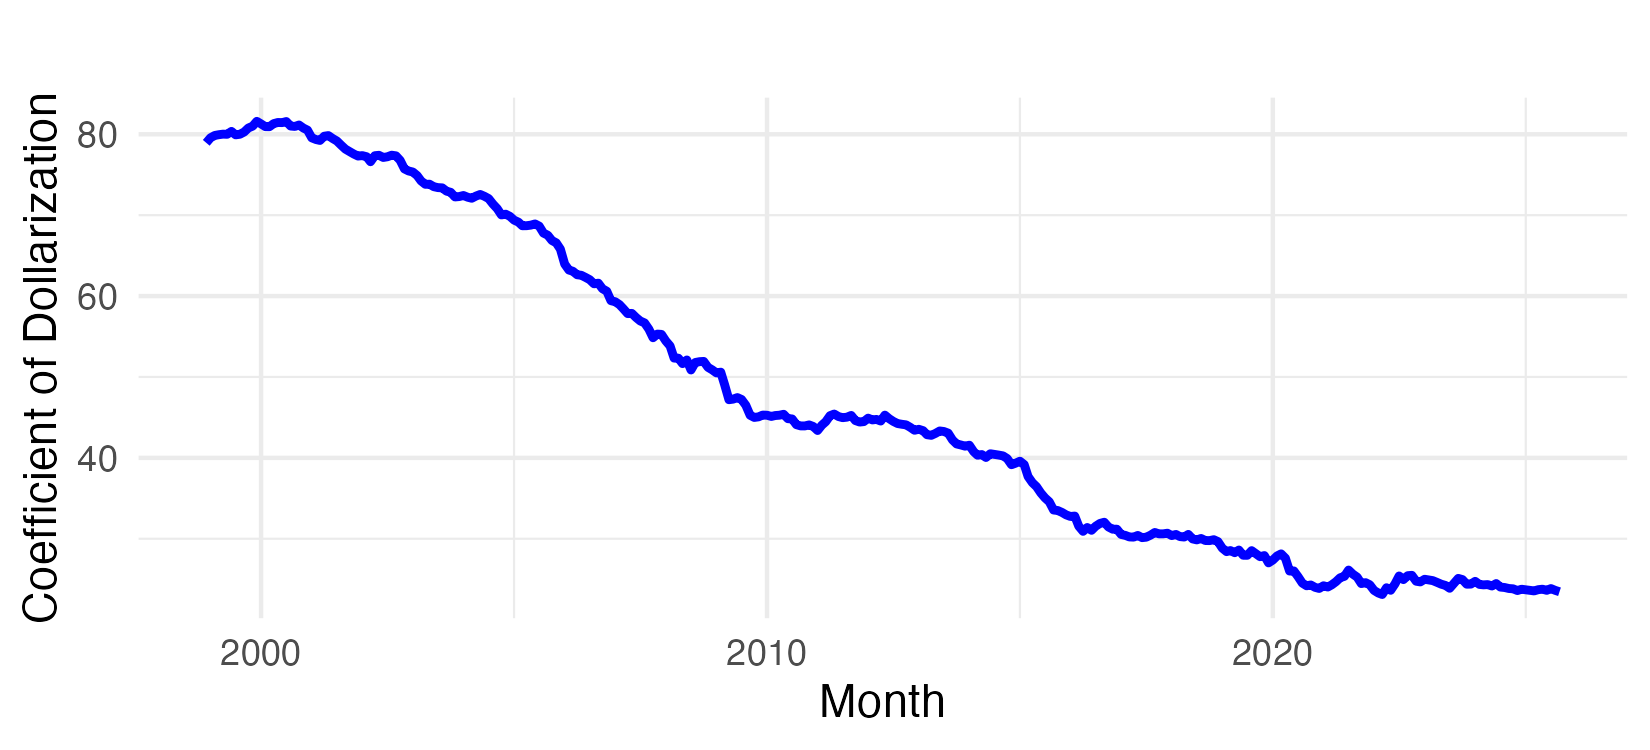
\includegraphics[width=0.85\linewidth]{figures/doll_plot.png }     
    \label{fig:doll_plot}
 \end{figure}


\begin{figure}[H]
    \centering
    \caption{Terms-of-trade pass-through to the exchange rate}
    \includegraphics[width=\linewidth]{figures/tot_passthrough.pdf }     
    \label{fig:tot_passthrough_plot}
 \end{figure}


\begin{table}[H]
    \centering
    \begin{singlespace}
    \caption{ToT pass-through: $\Delta \log e_t = \alpha + \beta \, \Delta \log (p_{im}/p_{ex})_t + \varepsilon_t$}
    \label{tab:tot_passthrough}
    \begin{tabular}{lc}
        \toprule
        & $\Delta \log e_t$ \\
        \midrule
        $\alpha$ & 0.0017 \\
                  & (0.0023) \\[4pt]
        $\beta$   & 0.1237 \\
                  & (0.0530) \\
        \midrule
        $R^2$     & 0.0522 \\
        $N$       & 101 \\
        \bottomrule
    \end{tabular}

    \smallskip
    \centering
    \begin{minipage}{0.5\linewidth}
    \footnotesize
    \textit{Notes:} OLS estimates. Standard errors in parentheses.
    \end{minipage}
    \end{singlespace}
\end{table}


\newpage
\bibliography{bibliography}
%TC:endignore

\end{document}

